\documentclass[11pt]{article}

\usepackage[margin=1in]{geometry}
\usepackage[T1]{fontenc}
\usepackage[utf8]{inputenc}
\usepackage{lmodern}
\usepackage{setspace}
\usepackage{amsmath,amssymb}
\usepackage{graphicx}
\usepackage{booktabs}
\usepackage{array}
\usepackage{tabularx}
\usepackage{longtable}
\usepackage{xcolor}
\usepackage[numbers,sort&compress]{natbib}
\usepackage[colorlinks=true,allcolors=blue]{hyperref}

\newcolumntype{Y}{>{\raggedright\arraybackslash}X}
\newcommand{\runname}[1]{\texttt{#1}}
\newcommand{\evidencefile}[1]{\path{#1}}

\title{Benchmarking Agentic Large Language Models for Complex Protein-Set Functional Annotation}
\author{Xiaoyu Zhang\textsuperscript{*}}
\date{}

\begin{document}

\maketitle

\begin{center}
Department of Computer Science and Engineering, California State University San Marcos, San Marcos, CA 92096, USA\\
\textsuperscript{*}Correspondence: xiaoyu@csusm.edu
\end{center}

\begin{abstract}
Large language model (LLM) agents are increasingly used to synthesize heterogeneous bioinformatics evidence, but their reliability for high-volume biological annotation remains poorly characterized. We evaluated three agent configurations on a controlled protein annotation task: Claude App with Claude Opus 4.7, Claude Code CLI with Claude Opus 4.7 and Claude Scientific Skills, and Codex App with GPT-5.4 and Claude Scientific Skills. Each configuration was run three times on the same verbatim prompt, the same 73 selected orthogroup FASTA files (1{,}705 protein sequences), and the same local evidence: Swiss-Prot BLASTP output, Pfam/HMMER domain hits, DeepTMHMM topology predictions, and SignalP secretion predictions. We audited the nine outputs for coverage, biological correctness, missing evidence, hallucinated or over-specific annotations, and within-method consistency, then merged the best-supported evidence into a final orthogroup annotation table. All nine runs covered all 73 orthogroups, indicating that the agents could retrieve and organize the complete input set. However, normalized calcification-relevance calls were only moderately reproducible: within-method exact tier agreement ranged from 0.397 to 0.685 for Claude App (mean 0.562), 0.342 to 0.740 for Claude Code (mean 0.516), and 0.411 to 0.630 for Codex App (mean 0.539), and the per-run number of high-confidence calls varied from 0 to 12 across the nine runs. The final curated table retained 3 high-confidence, 9 moderate, 18 watchlist, and 43 low-relevance orthogroups. The most robust direct candidates were sulfatase (OG0017138) and sulfotransferase (OG0020703) families and an FG-GAP/integrin-like surface protein family (OG0018986), whereas common error modes included overcalling pentapeptide-repeat proteins, weak secreted housekeeping enzymes, and low-complexity BLAST hits as calcification proteins. Skill-enabled agents improved file handling, evidence traceability, and reproducibility of computational checking, but they did not eliminate biological overinterpretation. These results support a best-practice workflow in which LLM agents draft annotations only after deterministic evidence tables are generated, with explicit scoring rules, provenance columns, run-to-run replication, and expert review of high-impact claims.
\end{abstract}

\doublespacing

\section{Introduction}

Protein function annotation is a persistent bottleneck in comparative genomics. Sequence databases now contain hundreds of millions of protein records, and even curated resources combine expert review, automated rule transfer, domain signatures, and machine-learning predictions to keep pace with new genomes \citep{UniProt2025}. Homology searches such as BLAST remain a practical first pass \citep{Altschul1990}, while profile-HMM domain searches against Pfam add family-level evidence that is often more sensitive for remote homologs \citep{Mistry2021,Eddy2011}. Secretion and membrane-topology predictors such as SignalP 6.0 and DeepTMHMM provide orthogonal context about whether a protein could act in extracellular matrices, vesicles, or membranes \citep{Teufel2022,Hallgren2022}. Combining these evidence streams is routine, but the final biological interpretation is still difficult because many protein families are multidomain, repetitive, lineage-specific, or only indirectly connected to the process of interest. Community-wide evaluations of automated function prediction have also shown that even the best classifiers fall well short of perfect agreement with expert-curated annotations, with reliability that varies systematically across functional categories and taxonomic groups \citep{Radivojac2013}.

The task considered here is especially challenging: annotating selected orthogroups for possible relevance to calcification. Coccolithophore calcification involves CaCO$_3$ scale formation, endomembrane trafficking, ion and proton handling, and organic matrix components \citep{Brownlee2015,Skeffington2023}. Coccolith-associated polysaccharides can contain acidic and sulfated residues and influence calcite crystal morphology \citep{Kayano2011}. Therefore, sulfation, glycosylation, secreted matrix proteins, adhesion proteins, transporters, and vesicle-associated factors can all be biologically plausible. At the same time, the same vocabulary creates a high risk of false positives: a generic secreted enzyme, a single weak collagen-like BLAST hit, or a calcium-binding domain in an unrelated intracellular protein should not automatically be called a calcification factor.

Agentic LLM systems appear attractive for such annotation because they can read many files, summarize evidence, write reports, and in coding environments run scripts to check their own outputs. Claude Code is described by Anthropic as an agentic coding tool that can read a codebase, edit files, run commands, and integrate with development tools \citep{AnthropicClaudeCode2026}. OpenAI describes Codex as a coding agent that can read, edit, and run code, including background and parallel cloud tasks \citep{OpenAICodex2026}. Scientific skill libraries add domain-specific instructions, examples, and workflow scaffolds; the K-Dense Scientific Agent Skills repository currently describes a collection of ready-to-use scientific and research skills for agent systems \citep{KDenseSkills2026}. These capabilities may improve the mechanics of scientific workflows, but they do not by themselves guarantee biological correctness.

Here we use a controlled, repeated-run comparison to evaluate three agent configurations as they were used on the same orthogroup annotation prompt. The goal is not to rank proprietary foundation models in general. Instead, we ask a practical question relevant to bioinformatics groups: when agents are asked to retrieve, integrate, and interpret a large set of complex protein annotations, where do they help, where do they fail, how consistent are repeated runs, and how should their outputs be merged into a defensible final annotation table?

\section{Results}

\subsection{All agents completed the retrieval task, but interpretation varied substantially}

Each of the nine runs returned annotations for all 73 orthogroups, so no method failed at the basic retrieval and coverage layer. The shared input comprised 1,705 protein sequences, 73 BLAST tables, 73 Pfam/HMMER tables, seven DeepTMHMM topology batches, and two SignalP batches. The downstream differences therefore reflected how the agents interpreted evidence rather than whether they found the files.

The final expert-audited merge classified 3 orthogroups as high relevance, 9 as moderate relevance, 18 as watchlist candidates, and 43 as low relevance (Figure~\ref{fig:workflow}). The high-confidence set was intentionally conservative. It included OG0017138, an arylsulfatase/sulfatase family; OG0020703, a heparan-sulfate or sulfoglycan sulfotransferase-like enzyme; and OG0018986, an FG-GAP/integrin-alpha-like cell-surface receptor family with secretion or membrane-topology support. Moderate candidates were retained when evidence supported an indirect or plausible matrix, polysaccharide, surface, or remodeling role but lacked enough family-wide specificity for a high-confidence call.

\begin{figure}[ht]
  \centering
  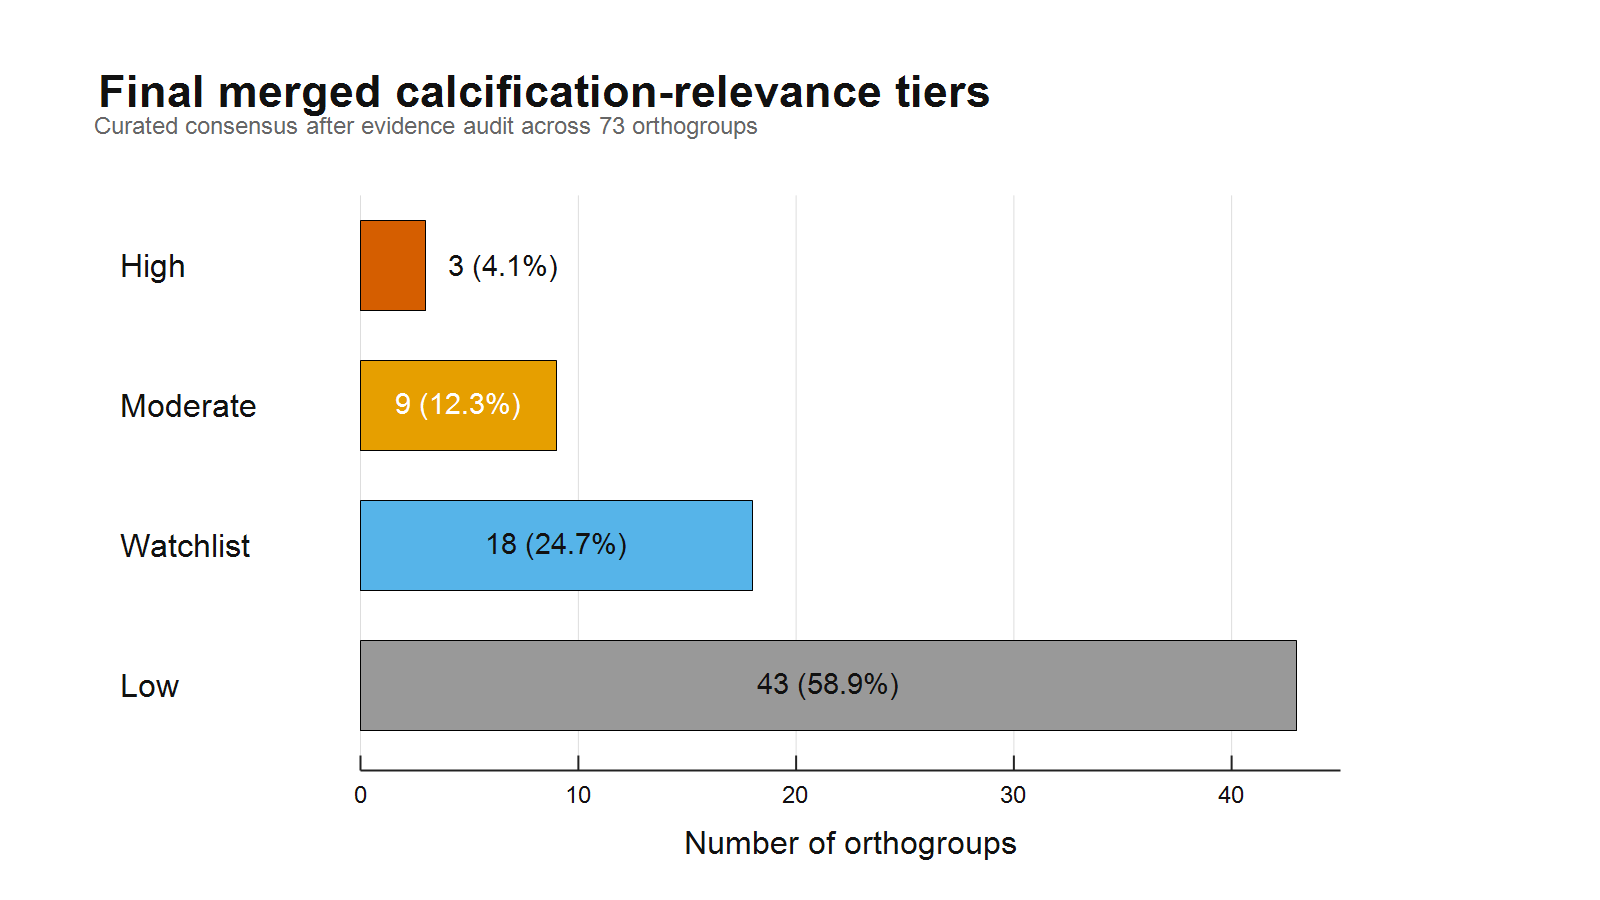
\includegraphics[width=0.88\linewidth]{figures/final_relevance_distribution.png}
  \caption{Final curated calcification-relevance distribution after the controlled benchmark workflow. The shared input consisted of 73 orthogroup FASTA files with Swiss-Prot BLASTP, Pfam/HMMER, DeepTMHMM, and SignalP evidence. Three independent runs were performed for each agent configuration: Claude App Opus 4.7, Claude Code Opus 4.7 with scientific skills, and Codex App GPT-5.4 with scientific skills. Model outputs were normalized to common relevance tiers, checked against recomputed evidence summaries, audited for overcalls and missing evidence, and merged into the final annotation table.}
  \label{fig:workflow}
\end{figure}

\subsection{Run-level calibration differed within and between methods}

Although coverage was complete, calibration differed strongly across runs (Figure~\ref{fig:run_distribution}; Table~\ref{tab:runs}). Claude App run 2 was highly conservative, assigning 67 of 73 orthogroups to a low or background tier and only one high call. Claude App runs 1 and 3 were less conservative, with 11 and 8 high calls, respectively. Claude Code with scientific skills produced fewer high calls overall (1, 3, and 2), but shifted substantially between low and watchlist labels across runs. Codex App with scientific skills showed the widest high-call range, from no high calls in run 2 to 12 high calls in run 3.

\begin{figure}[ht]
  \centering
  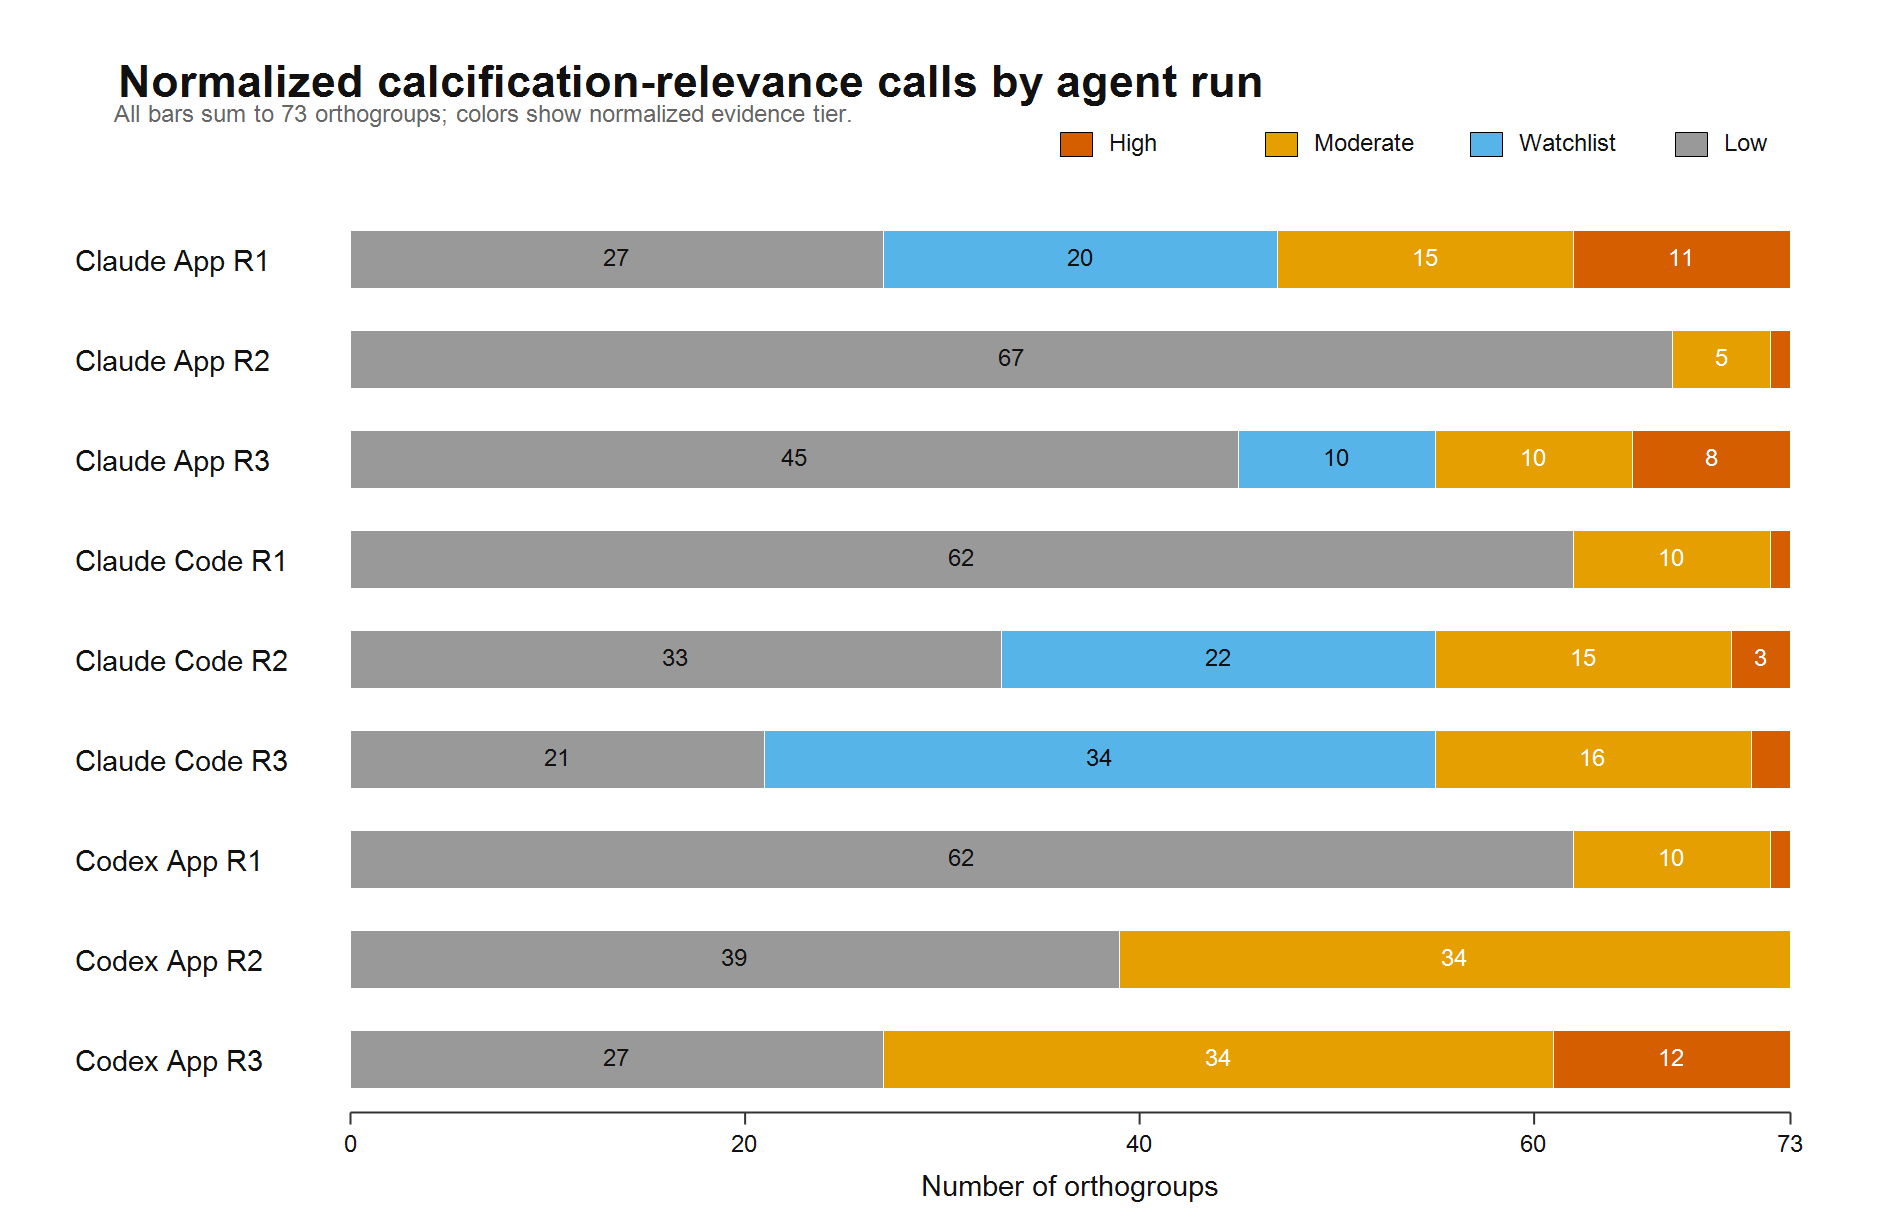
\includegraphics[width=\linewidth]{figures/run_relevance_distribution.png}
  \caption{Normalized calcification-relevance distributions for the nine agent runs. Each horizontal bar sums to the 73 shared orthogroups, showing that all runs had complete coverage but differed substantially in calibration.}
  \label{fig:run_distribution}
\end{figure}

\begin{table}[ht]
\centering
\small
\caption{Run-level relevance calibration after normalization of each output to common evidence tiers.}
\label{tab:runs}
\begin{tabularx}{\linewidth}{lrrrrrY}
\toprule
Run & High & Moderate & Watchlist & Low & Mean score & Main calibration pattern\\
\midrule
\runname{Claude\_app\_run1} & 11 & 15 & 20 & 27 & 1.71 & Broadly permissive; many secreted or membrane families promoted.\\
\runname{Claude\_app\_run2} & 1 & 5 & 0 & 67 & 0.68 & Most conservative output; few indirect candidates retained.\\
\runname{Claude\_app\_run3} & 8 & 10 & 10 & 45 & 1.29 & Intermediate, but still promoted several weak matrix candidates.\\
\runname{Claude\_code\_run1} & 1 & 10 & 0 & 62 & 0.82 & Conservative and similar to \runname{Codex\_app\_run1}.\\
\runname{Claude\_code\_run2} & 3 & 15 & 22 & 33 & 1.36 & Better separation of watchlist from low, but still some overcalls.\\
\runname{Claude\_code\_run3} & 2 & 16 & 34 & 21 & 1.50 & Most watchlist-heavy Claude Code output.\\
\runname{Codex\_app\_run1} & 1 & 10 & 0 & 62 & 0.82 & Conservative baseline-like output.\\
\runname{Codex\_app\_run2} & 0 & 34 & 0 & 39 & 1.43 & Broad plausible-indirect labeling with no high tier.\\
\runname{Codex\_app\_run3} & 12 & 34 & 0 & 27 & 2.01 & Most permissive run; many indirect candidates promoted.\\
\bottomrule
\end{tabularx}
\end{table}

Two additional calibration patterns stood out. First, Codex App never emitted a watchlist-tier label in any of its three runs, instead splitting every orthogroup among high, moderate, and low tiers; this is a vocabulary choice rather than a coverage failure, but it forced the normalization step to re-bucket moderate Codex calls that functionally behaved like watchlist candidates, and it prevented Codex from marking orphan-secreted or orphan-membrane families as explicitly provisional. Second, Claude Code run 1 and Codex App run 1 produced identical normalized distributions (high=1, moderate=10, low=62), despite coming from different model families and different agent interfaces; this apparent convergence on a conservative baseline under stochastic decoding suggests that when the prompt is interpreted literally, both agent families default to a similar ``only call what is directly evidenced'' pattern.

Within-method exact agreement on normalized relevance labels was modest (Figure~\ref{fig:within_agreement}; Table~\ref{tab:agreement}). The best agreement was between Claude Code runs 2 and 3 (54/73 orthogroups; 0.740), while the lowest was between Claude Code runs 1 and 3 (25/73; 0.342). Mean within-method agreement was in the same range for all three configurations (0.516--0.562), so no configuration was dramatically more reproducible than the others at the tier-label level. These results argue against relying on a single stochastic agent run for final biological claims, even when the input files and prompt are identical.

\begin{table}[ht]
\centering
\small
\caption{Within-method exact agreement between repeated runs after tier normalization.}
\label{tab:agreement}
\begin{tabular}{lccc}
\toprule
Method & Run-pair agreements & Mean agreement & Range\\
\midrule
Claude App Opus 4.7 & 0.397, 0.603, 0.685 & 0.562 & 0.397--0.685\\
Claude Code Opus 4.7 + skills & 0.466, 0.342, 0.740 & 0.516 & 0.342--0.740\\
Codex App GPT-5.4 + skills & 0.630, 0.411, 0.575 & 0.539 & 0.411--0.630\\
\bottomrule
\end{tabular}
\end{table}

\begin{figure}[ht]
  \centering
  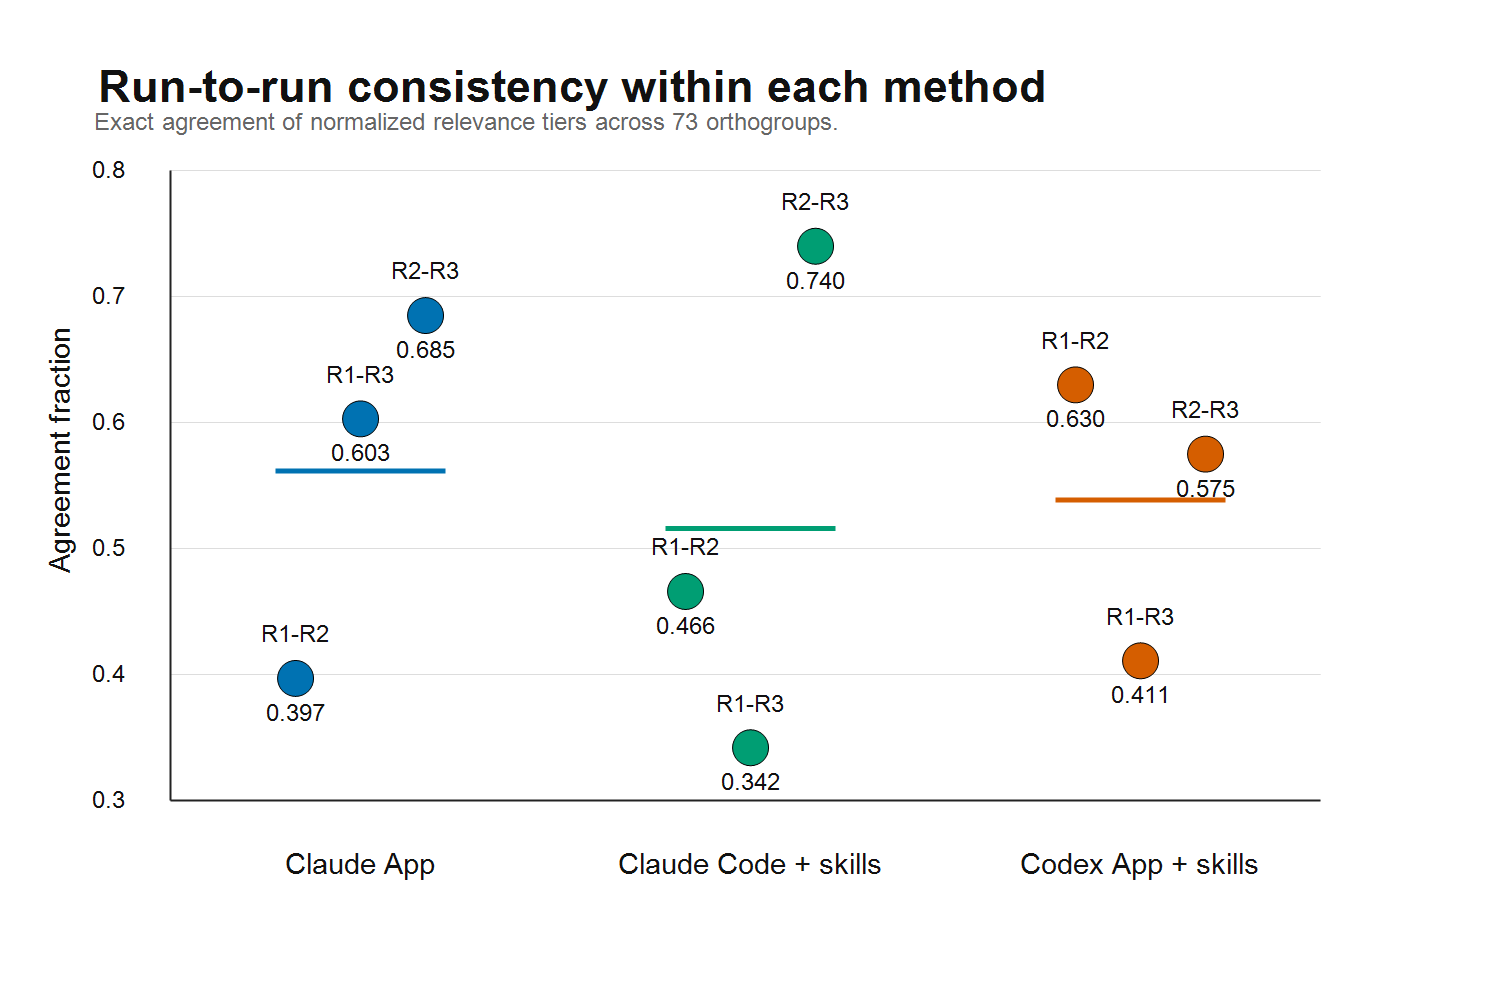
\includegraphics[width=0.92\linewidth]{figures/within_method_agreement.png}
  \caption{Pairwise run-to-run consistency within each method. Dots show exact normalized-tier agreement for each pair of repeated runs; horizontal lines show the method mean.}
  \label{fig:within_agreement}
\end{figure}

\subsection{Biologically robust candidates shared direct matrix-chemistry or surface evidence}

The final high-confidence candidates were those for which the evidence connected directly to known features of calcification biology rather than only to generic secretion or membrane localization (Table~\ref{tab:candidates}). OG0017138 had strong family-wide sulfatase support, with 14 of 16 sequences carrying a Sulfatase Pfam hit (best $E$-value $4.6\times10^{-48}$) and all 16 sequences mapping to arylsulfatase BLAST hits. OG0020703 combined a coherent though more sparsely covered sulfotransferase signal (1 of 11 sequences with a Sulfotransfer\_1/Sulfotransfer\_3 Pfam hit and 2 of 11 with heparan-sulfate-6-$O$-sulfotransferase BLAST hits) with family-wide secretion support (4/11 SignalP-positive; no predicted transmembrane regions) in an orthogroup size small enough that a family-level sulfotransferase assignment is reasonable. These functions are biologically coherent because coccolith-associated polysaccharides include acidic and sulfated components that can influence calcium carbonate crystallization \citep{Kayano2011}. OG0018986 was retained as high because it combined family-wide FG-GAP repeats (12 of 13 sequences with FG-GAP and FG-GAP\_3 Pfam hits) with extracellular or membrane topology (7/13 SignalP-positive, 10/13 with predicted transmembrane or SP+TM topology). This is not a direct enzyme in carbonate chemistry, but it is one of the strongest non-enzymatic surface or adhesion candidates in the dataset.

\begin{table}[ht]
\centering
\small
\caption{Final high and moderate calcification-relevance candidates after evidence audit.}
\label{tab:candidates}
\begin{tabularx}{\linewidth}{p{1.7cm}p{1.0cm}p{4.7cm}Y}
\toprule
Tier & Count & Orthogroups & Evidence basis\\
\midrule
High & 3 & OG0017138; OG0018986; OG0020703 & Direct sulfatase or sulfotransferase chemistry tied to sulfated matrix glycans, plus one FG-GAP/integrin-like surface family with strong topology and domain support.\\
Moderate & 9 & OG0009246; OG0009301; OG0009816; OG0011061; OG0017305; OG0021347; OG0023594; OG0024846; OG0025059 & Secreted adhesive or orphan proteins, glycosyltransferase-like enzymes, sulfotransferase with limited coverage, and secreted protease or proline/cysteine-rich matrix candidates.\\
Watchlist & 18 & See final TSV & Orphan secreted or membrane families, membrane organizers, signaling proteins, or weakly supported matrix-like families requiring follow-up evidence.\\
Low & 43 & See final TSV & Housekeeping, intracellular, weakly annotated, or unsupported families without calcification-specific evidence.\\
\bottomrule
\end{tabularx}
\end{table}

The moderate tier was deliberately heterogeneous. For example, OG0009816, OG0011061, OG0023594, and OG0024846 were glycosyltransferase-like candidates with plausible links to matrix or cell-wall polysaccharide biosynthesis, but their evidence was too indirect or incomplete for a high call. OG0025059 was a strong novel secreted orphan candidate, with five of seven SignalP-positive sequences and no transmembrane prediction, but it lacked a functional domain. Such proteins are valuable experimental targets but should be annotated as candidates rather than known calcification proteins.

The evidence heatmap in Figure~\ref{fig:candidate_heatmap} shows why the final high and moderate candidates could not be treated as a single homogeneous class. Some orthogroups had strong family-wide BLAST and Pfam support, while others were retained primarily because of secretion or membrane topology. The heatmap also highlights cases with high model consensus but limited domain coverage, which were the cases most likely to require manual downgrading.

\begin{figure}[ht]
  \centering
  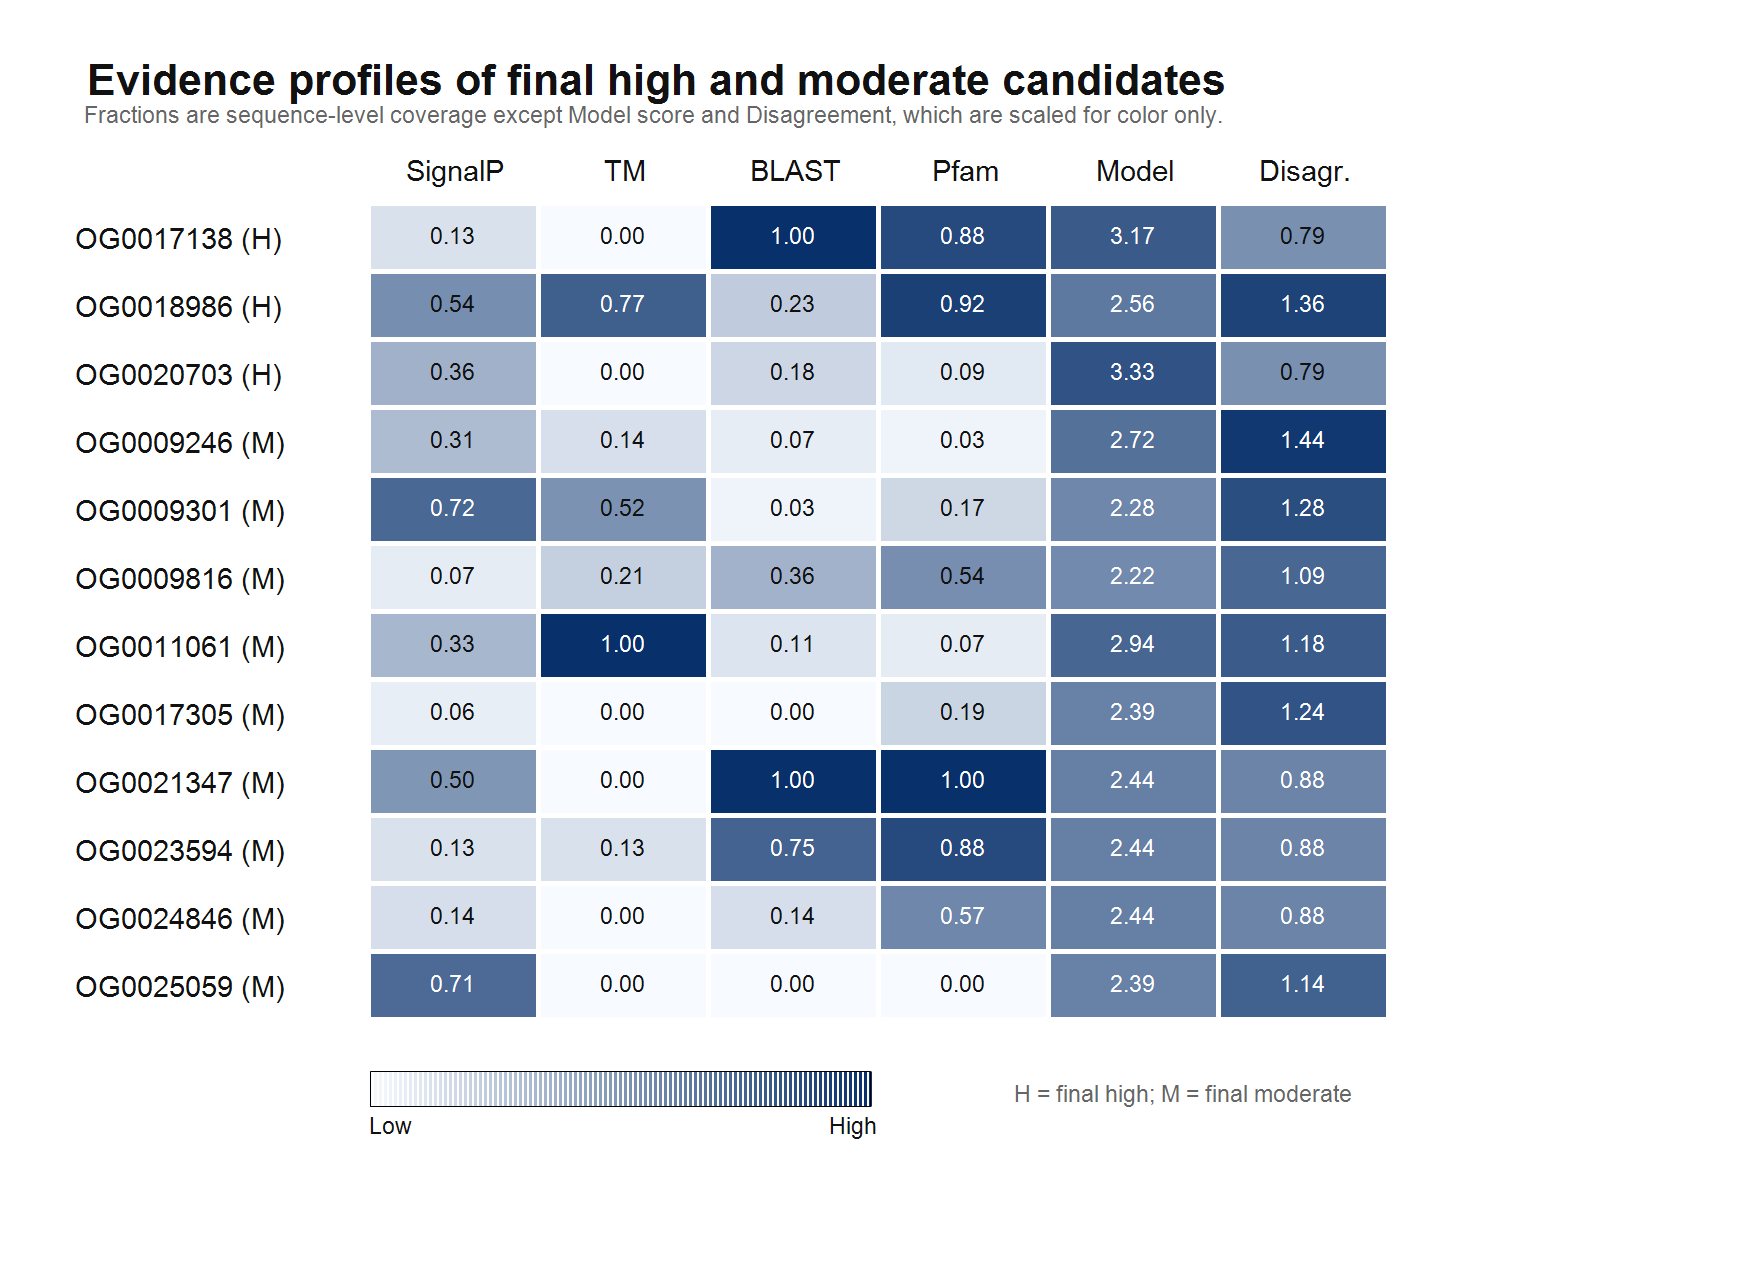
\includegraphics[width=\linewidth]{figures/candidate_evidence_heatmap.png}
  \caption{Evidence profiles for final high and moderate candidates. SignalP, TM, BLAST, and Pfam columns show sequence-level fractions. Model is the mean normalized model relevance score, and disagreement is the between-run standard deviation; these two columns are numerically labeled with their raw values but color-scaled for display.}
  \label{fig:candidate_heatmap}
\end{figure}

\subsection{Common hallucination and overclaim modes were biologically interpretable}

The most important error mode was not invented file content but over-specific biological inference from real but weak evidence. Pentapeptide-repeat orthogroups (OG0001976, OG0010867, and OG0022524) were repeatedly elevated by some runs despite strong local evidence only for pentapeptide repeats, mostly globular topology, and no direct calcification marker; pentapeptide-repeat proteins are characterized by a right-handed quadrilateral $\beta$-helical (Rfr) fold and have no known calcium- or carbonate-binding activity \citep{Vetting2006}. Several secreted housekeeping enzymes were similarly overranked when secretion was treated as sufficient evidence for matrix function. Low-complexity or repetitive BLAST hits also misled some outputs: the DNA-directed RNA polymerase II subunit RPB1 hit for OG0009301, Piccolo-like hits for OG0011061 or OG0015153, and a collagen call for OG0016203 based on one member of an 18-sequence family all required downgrading.

These mistakes mirror known issues in automated protein annotation. Public databases and computational transfer pipelines can accumulate overprediction and misannotation when specific functions are assigned beyond the support provided by family-level evidence \citep{Schnoes2009}. LLM agents add an additional layer: they can produce fluent rationales that make weak annotation transfer sound mechanistically complete. For this dataset, the safer interpretation rule was to annotate at the specificity level actually supported by BLAST, Pfam, topology, secretion, and family-wide coverage.

\subsection{Scientific skills improved workflow mechanics more than biological calibration}

This benchmark cannot isolate skills as an independent causal variable because the skill-enabled conditions also used different interfaces from Claude App, and Codex used a different model family. Nevertheless, the qualitative comparison is informative. The skill-enabled coding-agent runs were better suited to deterministic checks: they could inspect folders, aggregate evidence, write scripts, and produce reproducible TSV outputs. That advantage was important for coverage checking and provenance, and it made it easier to diagnose disagreements after the fact.

However, the presence of scientific skills did not guarantee conservative biological judgment. Claude Code produced both conservative and watchlist-heavy outputs, while Codex ranged from conservative to highly permissive. This suggests that skills help agents use tools and domain workflows, but final biological calibration still depends on explicit prompt constraints, scoring rules, and review. In other words, skills improved the annotation process, but not enough to replace an evidence audit.

\section{Discussion}

The primary lesson from this benchmark is that agentic LLMs are useful assistants for protein-set annotation, but they should be treated as evidence organizers and hypothesis generators, not autonomous curators. All three agent configurations found and processed the complete orthogroup set. This is a meaningful practical success for large annotation folders, where failures often arise from missed files, inconsistent filenames, or incomplete output tables. The agents also surfaced plausible biology, especially sulfation, glycosylation, secreted orphan proteins, and membrane candidates.

The main weakness was calibration. The same prompt and same evidence produced runs that ranged from one high-confidence candidate to twelve. The final manual merge retained only three high-confidence orthogroups, indicating that several runs overestimated calcification relevance. The most permissive outputs were not useless; they often identified good watchlist candidates. Their problem was that they blurred the distinction between direct evidence, indirect pathway plausibility, and speculative follow-up.

For similar bioinformatics tasks, we recommend a staged workflow. First, generate deterministic evidence tables before asking an LLM for interpretation. Each orthogroup should have sequence counts, species counts, BLAST hit coverage, Pfam hit coverage, best E-values, SignalP fractions, DeepTMHMM topology summaries, and any low-complexity or single-member caveats. Second, require agents to assign both a function label and an evidence tier, with explicit definitions for high, moderate, watchlist, and low. Third, run the same prompt multiple times or across agents, then inspect disagreements rather than averaging them away. Fourth, include a negative-control mindset: housekeeping enzymes, single-hit collagen labels, repetitive proteins, and generic secretion should be downgraded unless supported by family-wide domains or process-specific biology. Finally, reserve final labels such as ``calcification protein'' for experimentally supported genes or very strong mechanistic evidence; use ``candidate'', ``watchlist'', or ``indirectly relevant'' for the more common cases.

The comparison also suggests that skill libraries are most valuable when they push agents toward reproducible computation. Skills should include templates for evidence schemas, scripts for re-aggregating annotation files, checks for missing orthogroups, and prompts that force conservative interpretation of weak homology. They should not only provide domain vocabulary, because vocabulary without calibration can increase overconfident mechanistic narratives.

\subsection{Limitations}

Several limitations of this benchmark should be kept in mind when generalizing from the results. First, the three agent configurations differ in more than one axis at once: Claude App uses a chat-style interface without a local code-execution environment, while Claude Code and Codex App run in coding-agent interfaces with local file and shell access, and only two of the three conditions use the scientific skill library. We therefore cannot cleanly attribute observed differences to model family, interface, or skill library as independent factors. Second, we ran each configuration only three times, which is sufficient to show that single-run biological conclusions are unstable but too small to support quantitative inference on reproducibility differences between configurations; larger replicate counts would be required to claim, for example, that Claude App is reliably more or less consistent than Codex App. Third, the benchmark target is calcification relevance in one taxonomic context, and the error modes observed here (over-reading pentapeptide repeats, housekeeping secreted enzymes, and low-complexity BLAST labels) may be more or less prominent in other biological tasks. Fourth, the curated merge is itself an expert judgment rather than a held-out ground truth, so ``overcalling'' and ``undercalling'' should be read relative to a defensible conservative standard, not as errors against a gold label. Fifth, the relevance categories we report are ordinal but coarse; a finer-grained scoring rubric, or quantitative evidence-weight features, could reduce inter-run variability that comes purely from threshold drift between runs.

\section{Methods}

\subsection{Input data and agent configurations}

The benchmark used the folder \evidencefile{Orthogroups.calcifying\_loose\_fastas}, which contained 73 selected orthogroup FASTA files spanning 1{,}705 protein sequences from a comparative coccolithophore proteome. Each method received the same verbatim prompt asking it to annotate the biological function of each orthogroup, assess relevance to calcification, and use the local BLASTP, Pfam/HMMER, DeepTMHMM, and SignalP outputs in the same input directory; agents were also permitted to generate additional supporting evidence if they judged it necessary. The three evaluated configurations were: Claude App with Claude Opus 4.7 \citep{AnthropicOpus47_2026} at the highest available reasoning setting; Claude Code CLI with Claude Opus 4.7 at the highest available reasoning setting and the Claude Scientific Skills library; and Codex App with GPT-5.4 at the highest available reasoning setting and the same scientific skill library. Each configuration was run three independent times with no inter-run state, conversation history, or shared scratchpad.

\subsection{Evidence audit and normalization}

After the nine outputs were produced, we recomputed orthogroup-level evidence summaries from the local files. BLAST and Pfam results were summarized by number of query sequences with hits, top hit labels, domain labels, and best E-values. SignalP outputs were summarized as counts and fractions of proteins with predicted signal peptides. DeepTMHMM outputs were summarized as globular, secreted, transmembrane, or secreted-plus-transmembrane categories and by transmembrane-region counts. These summaries were written to \evidencefile{recomputed\_evidence.tsv} in the comparison output directory.

Model relevance labels used different vocabularies, so each call was mapped to a common ordinal tier: low/background/unlikely, watchlist/uncertain, moderate/possible/plausible, and high/direct. We then calculated per-orthogroup mean score, score range, score standard deviation, overcalling runs, and undercalling runs in \evidencefile{comparison\_merged\_annotation/model\_run\_comparison.tsv}. Within-method consistency was measured as exact agreement between normalized tier labels for each pair of repeated runs.

\subsection{Final annotation merge}

The final table was curated from three information sources: the recomputed evidence table, the nine model outputs, and manual biological review of disagreement cases. We favored family-wide domain and topology support over isolated hits. We classified an orthogroup as high relevance only when the evidence was both strong and mechanistically close to calcification chemistry, matrix biology, or surface adhesion. Moderate relevance required plausible but incomplete or indirect evidence. Watchlist status was used for orphan secreted or membrane families and weakly connected signaling or vesicle candidates. Low relevance was assigned to housekeeping, intracellular, unsupported, or weakly annotated families without a specific calcification link. The final output was written to \evidencefile{final\_orthogroup\_annotations.tsv} in the comparison output directory.

\section{Conclusion}

In this controlled annotation task, agentic LLMs were effective at gathering and presenting evidence across dozens of orthogroups, but their biological conclusions were not stable enough to accept without curation. The same prompt and the same evidence produced runs that varied between one and twelve high-confidence calls, and only three orthogroups survived the conservative merge as direct calcification candidates: an arylsulfatase family (OG0017138), a heparan-sulfate-like sulfotransferase family (OG0020703), and an FG-GAP/integrin-like surface-receptor family (OG0018986). Scientific skills and coding-agent interfaces improved reproducibility and provenance, especially by enabling local evidence aggregation, but they did not remove the need for explicit scoring rules and expert review. The strongest practical design is therefore a hybrid one: deterministic bioinformatics evidence generation, replicated agent interpretation, automated disagreement detection, and conservative expert adjudication before final labels are used for downstream biology.

\section{Data and Code Availability}

All benchmark inputs and outputs analyzed here are local to the project workspace. The merged annotation and comparison files are available in \evidencefile{comparison\_merged\_annotation/}. Key files include:
\begin{itemize}
  \item \evidencefile{final\_orthogroup\_annotations.tsv}
  \item \evidencefile{model\_run\_comparison.tsv}
  \item \evidencefile{method\_consistency\_summary.tsv}
  \item \evidencefile{recomputed\_evidence.tsv}
\end{itemize}
The manuscript source is in \evidencefile{main.tex}; the bibliography is in \evidencefile{references.bib}.

\section{Acknowledgments}

The author thanks the developers and maintainers of the bioinformatics tools and databases used as evidence sources, including UniProt, BLAST, Pfam, HMMER, SignalP, and DeepTMHMM.

\section{Funding}

No specific funding was declared for this manuscript draft.

\section{Author Contributions}

X.Z. designed the benchmark, generated or collected the agent outputs, performed the comparative audit, curated the final annotation table, and wrote the manuscript.

\section{Competing Interests}

The author declares no competing interests.

\bibliographystyle{unsrtnat}
\bibliography{references}

\clearpage
\appendix
\singlespacing
\renewcommand{\thetable}{S\arabic{table}}
\renewcommand{\thefigure}{S\arabic{figure}}
\renewcommand{\theHtable}{S\arabic{table}}
\renewcommand{\theHfigure}{S\arabic{figure}}
\setcounter{table}{0}
\setcounter{figure}{0}

\section*{Supplementary Information}
\addcontentsline{toc}{section}{Supplementary Information}

Supplementary Table~\ref{tab:s_final_annotations} provides the complete final merged annotation table for all 73 orthogroups. Supplementary Table~\ref{tab:s_method_summary} gives the full method-level run summary, and Supplementary Table~\ref{tab:s_pairwise_agreement} lists the pairwise run-to-run agreement values underlying Figure~\ref{fig:within_agreement}.

\begingroup
\footnotesize
\setlength{\tabcolsep}{3pt}
\begin{longtable}{p{1.9cm}r p{4.55cm}p{1.8cm}p{5.55cm}}
\caption{Complete final merged annotations for the 73 orthogroups. The table is derived from \texttt{final\_orthogroup\_annotations.tsv}.}\label{tab:s_final_annotations}\\
\toprule
Orthogroup & n & Final function & Relevance & Curated rationale\\
\midrule
\endfirsthead
\caption[]{Complete final merged annotations for the 73 orthogroups (continued).}\\
\toprule
Orthogroup & n & Final function & Relevance & Curated rationale\\
\midrule
\endhead
\midrule
\multicolumn{5}{r}{Continued on next page}\\
\endfoot
\bottomrule
\endlastfoot
OG0000049 & 502 & Heterogeneous FKBP15/coiled-coil-like expanded family & Low & Very low BLAST/PFAM coverage and mostly globular; no calcification-specific evidence.\\
OG0001332 & 91 & Hint-domain or Hedgehog-Warthog-like membrane autoprocessing proteins & Watchlist & Strong Hint-domain and membrane topology support cell-surface signalling, but not a direct mineral-matrix function.\\
OG0001976 & 73 & Pentapeptide-repeat protein family & Low & Strong pentapeptide-repeat support, mostly non-secreted; no direct calcification evidence in the provided data.\\
OG0002887 & 59 & PIF1-family DNA helicase & Low & Housekeeping genome-maintenance helicase.\\
OG0003717 & 51 & Uncharacterized family & Low & No BLAST/PFAM annotation and weak TM signal only.\\
OG0009246 & 29 & Secreted adhesive or ECM-like protein family with weak collagen/adhesive BLAST support & Moderate & SignalP enrichment and adhesive/collagen BLAST hits make this a matrix candidate, but PFAM support is poor and homology coverage is low.\\
OG0009301 & 29 & Secreted or membrane-anchored proline-rich/SHOCT-like surface protein & Moderate & Very strong SignalP and membrane-anchor topology; RPB1 BLAST is likely low-complexity noise. Good surface/matrix candidate but no specific calcification domain.\\
OG0009816 & 28 & Golgi alpha-1,3-mannosyltransferase-like enzyme & Moderate & Mannosyltransferase PFAM and BLAST support glycosylation of secretory or matrix molecules, an indirect calcification-relevant process.\\
OG0010177 & 28 & Ankyrin-repeat scaffold protein & Low & Intracellular scaffold-like annotation with no secretion or calcification-specific evidence.\\
OG0010867 & 27 & Pentapeptide-repeat protein family & Low & Pentapeptide-repeat support but no strong secretion or mineralization-specific evidence.\\
OG0010991 & 27 & Uncharacterized family with minor secretion signal & Watchlist & No functional annotation; 4/27 SignalP positives make it a weak orphan follow-up, not a functional calcification call.\\
OG0011061 & 27 & Exostosin/GT47-like membrane glycosyltransferase candidate & Moderate & All proteins are membrane-associated and two have GT47 support; plausible polysaccharide/matrix biosynthesis role, but low PFAM coverage prevents a high-confidence direct call.\\
OG0011197 & 27 & 2OG-Fe(II) oxygenase or RAP-like protein & Low & Weak oxygenase support and top hits do not indicate matrix hydroxylation or calcification.\\
OG0013037 & 24 & Weak serine hydrolase or aminopeptidase-like family & Low & Sparse PFAM/BLAST support and mixed topology; no calcification-specific signal.\\
OG0014155 & 22 & Secreted or lumenal inosine-uridine nucleoside hydrolase & Watchlist & Strong secretion signal is notable, but enzyme chemistry is nucleotide salvage rather than matrix formation.\\
OG0014250 & 22 & Amidase or Glu-tRNA(Gln) amidotransferase-like enzyme & Low & High SignalP fraction but annotation points to general amidase/translation-related chemistry, not calcification.\\
OG0015153 & 20 & Unresolved multi-pass membrane protein family & Watchlist & Strong membrane topology with poor homology support makes it an orphan membrane candidate.\\
OG0016203 & 18 & Mostly membrane protein family with one collagen/RCC1-like member & Watchlist & One sequence has collagen-repeat evidence and most are TM, but family-wide collagen support is weak.\\
OG0016211 & 18 & SUR7/PalI-family multi-pass membrane organizer & Watchlist & All proteins are TM; membrane organization could matter for vesicle biology but no direct calcification marker is present.\\
OG0017138 & 16 & Arylsulfatase/sulfatase family & High & Strong family-wide Sulfatase PFAM and arylsulfatase BLAST support; sulfated polysaccharide remodeling is directly relevant to coccolith/matrix chemistry.\\
OG0017238 & 16 & tRNA ligase & Low & Housekeeping RNA-processing enzyme.\\
OG0017305 & 16 & Stf0-like sulfotransferase & Moderate & Sulfotransferase PFAM suggests sulfated matrix/glycan chemistry, but only 3/16 PFAM hits and SignalP support is weak by SignalP.\\
OG0017361 & 16 & DJ-1/PfpI family stress or cysteine hydrolase & Low & Stress/metabolic protein family with no specific mineralization link.\\
OG0017362 & 16 & Red chlorophyll catabolite reductase-like protein & Low & Plastid/chlorophyll-catabolism-like evidence despite partial SignalP.\\
OG0017884 & 15 & GNAT acetyltransferase & Low & General acetyltransferase with no calcification-specific evidence.\\
OG0017903 & 15 & Flavohemoprotein or oxidoreductase & Low & Redox/NO-detoxification-like function; no direct calcification evidence.\\
OG0017965 & 15 & Kelch/beta-propeller protein with possible NANM-like domain & Low & Likely intracellular/regulatory scaffold; no secretion or matrix evidence.\\
OG0018519 & 14 & Uncharacterized conserved multi-pass membrane family & Watchlist & 13/14 predicted TM and no homology; worth orphan membrane follow-up.\\
OG0018986 & 13 & FG-GAP/integrin-alpha-like cell-surface receptor with TM or 7TM features & High & Family-wide FG-GAP repeats plus secretion/TM topology support extracellular adhesion/Ca-binding receptor biology, one of the strongest non-enzymatic candidates.\\
OG0019067 & 13 & LRR/NLR-like receptor protein & Low & Immune/receptor-like LRR evidence, not specific to calcification.\\
OG0019078 & 13 & GST or elongation-factor-gamma-like protein & Low & Translation/redox housekeeping signal.\\
OG0019174 & 13 & Amidase or Glu-tRNA(Gln) amidotransferase-like enzyme & Low & Likely housekeeping amidase despite SignalP in some members.\\
OG0019180 & 13 & Uncharacterized soluble/orphan family & Low & No informative homology, domains, secretion, or TM signal.\\
OG0019790 & 12 & HECT E3 ubiquitin ligase with ankyrin repeats & Low & Protein-turnover scaffold, not calcification-specific.\\
OG0019817 & 12 & Secreted or lumenal FAD/NAD monooxygenase-like protein & Watchlist & SignalP enrichment is notable, but homology points to redox/secondary metabolism rather than matrix formation.\\
OG0019873 & 12 & Aminotransferase class I/II & Low & Generic metabolic enzyme.\\
OG0019887 & 12 & Ribosome-associated GTPase or intron maturase-like protein & Low & Organellar/ribosome-associated housekeeping evidence.\\
OG0019917 & 12 & Cyclic-nucleotide-binding or PKA-regulatory-like protein & Watchlist & cAMP signalling can regulate physiology, but evidence is indirect and not calcification-specific.\\
OG0020622 & 11 & RecD2/UvrD-like DNA helicase & Low & DNA repair helicase.\\
OG0020657 & 11 & Uncharacterized partially secreted family & Watchlist & No homology/domain support, but DeepTMHMM and SignalP suggest secretion in a subset.\\
OG0020696 & 11 & Uncharacterized weak membrane/secreted family & Watchlist & No homology/domain support and only partial topology signal.\\
OG0020700 & 11 & PDZ-domain scaffold protein & Low & Generic scaffold with no secretion or mineralization evidence.\\
OG0020703 & 11 & Heparan-sulfate or sulfoglycan sulfotransferase-like enzyme & High & Sulfotransferase BLAST/PFAM plus secretion support direct relevance to sulfated acidic matrix/polysaccharide chemistry.\\
OG0020706 & 11 & Uncharacterized multi-pass membrane family & Watchlist & No homology/domain support but 5/11 DeepTMHMM TM/SP+TM proteins.\\
OG0020728 & 11 & Uncharacterized soluble/orphan family & Low & No informative evidence.\\
OG0020729 & 11 & Uncharacterized soluble/orphan family & Low & No informative evidence.\\
OG0021347 & 10 & Secreted trypsin-family serine protease & Moderate & Strong trypsin PFAM plus secretion; matrix remodeling is plausible but indirect.\\
OG0021406 & 10 & Short-chain dehydrogenase or sugar-metabolism enzyme & Low & Metabolic enzyme with no calcification-specific evidence.\\
OG0021517 & 10 & F-box protein & Low & Protein-turnover adaptor.\\
OG0021520 & 10 & Mostly uncharacterized soluble family with one beta/TM outlier & Low & Topology support is not family-wide.\\
OG0021523 & 10 & PP2C protein phosphatase & Watchlist & Ca/Mg-dependent phosphatase chemistry is peripheral; no direct matrix/transport evidence.\\
OG0021531 & 10 & DegP/HtrA/PDZ protease-like protein & Low & Quality-control protease-like evidence with no SignalP support and no direct calcification link.\\
OG0022355 & 9 & Secreted/membrane DUF2237 protein family & Watchlist & Strong SP/TM topology and DUF support but no known calcification function.\\
OG0022381 & 9 & NADPH-cytochrome P450 reductase-like redox enzyme & Low & ER/redox metabolism, not calcification-specific.\\
OG0022455 & 9 & Uncharacterized soluble/orphan family & Low & No informative evidence.\\
OG0022473 & 9 & Uncharacterized partially secreted/membrane family & Watchlist & Partial topology signal without function; weak orphan candidate.\\
OG0022474 & 9 & F-box protein & Low & Protein-turnover adaptor.\\
OG0022492 & 9 & Beta-propeller/WD40 kinase-associated scaffold & Low & Regulatory scaffold/kinase hits, no calcification-specific evidence.\\
OG0022500 & 9 & Uncharacterized soluble/orphan family & Low & No informative evidence.\\
OG0022520 & 9 & Uncharacterized soluble/orphan family & Low & No informative evidence.\\
OG0022524 & 9 & Pentapeptide-repeat protein family & Low & Pentapeptide-repeat support but no secretion or direct calcification evidence.\\
OG0022528 & 9 & Uncharacterized soluble/orphan family & Low & No informative evidence.\\
OG0023496 & 8 & Protein kinase or GAK-BMP2K-like kinase & Watchlist & Possible vesicle/signalling role, but no direct mineral chemistry or matrix evidence.\\
OG0023566 & 8 & SEY1/RHD3-like ER-fusion GTPase & Low & Secretory/ER morphology role is broad, not calcification-specific.\\
OG0023594 & 8 & GT8 glycosyltransferase-like enzyme & Moderate & GT8 support is consistent with extracellular polysaccharide biosynthesis, a plausible matrix pathway.\\
OG0023657 & 8 & Uncharacterized soluble/orphan family & Low & No informative evidence.\\
OG0023790 & 8 & Red chlorophyll catabolite reductase-like protein & Low & Plastid/chlorophyll-catabolism-like evidence.\\
OG0024846 & 7 & TOD1/MUCI70-like hexosyltransferase & Moderate & MUCI70/TOD1 glycosyltransferase-like domain suggests matrix/cell-wall polysaccharide modification.\\
OG0024979 & 7 & Uncharacterized soluble/orphan family & Low & No informative evidence.\\
OG0025015 & 7 & Uncharacterized pan-calcifier multi-pass membrane family & Watchlist & 7/7 predicted TM and no homology; strong orphan transporter/membrane follow-up candidate.\\
OG0025016 & 7 & Uncharacterized soluble/orphan family & Low & No informative evidence.\\
OG0025059 & 7 & Uncharacterized secreted proline/cysteine-rich orphan protein & Moderate & 5/7 SignalP positives, no TM, no homology; classic novel secreted matrix-candidate profile but no functional domain.\\
OG0026865 & 6 & JmjC/cupin hydroxylase-like enzyme & Watchlist & Hydroxylase chemistry could affect matrix proteins, but evidence points broadly to JmjC/PSR-like enzymes and is indirect.\\
\end{longtable}
\endgroup


\begin{table}[ht]
\centering
\small
\caption{Full method-level consistency summary. Label distributions were normalized from each agent output.}
\label{tab:s_method_summary}
\begin{tabularx}{\linewidth}{lYrrr}
\toprule
Run & Normalized label distribution & Mean score & Score SD & Missing OGs\\
\midrule
\texttt{Claude\_app\_run1} & high=11; low=27; moderate/possible=15; watchlist/uncertain=20 & 1.71 & 1.22 & 0\\
\texttt{Claude\_app\_run2} & high=1; low=67; moderate/possible=5 & 0.68 & 0.64 & 0\\
\texttt{Claude\_app\_run3} & high=8; low=45; moderate/possible=10; watchlist/uncertain=10 & 1.29 & 1.19 & 0\\
\texttt{Claude\_code\_run1} & high=1; low=62; moderate/possible=10 & 0.82 & 0.79 & 0\\
\texttt{Claude\_code\_run2} & high=3; low=33; moderate/possible=15; watchlist/uncertain=22 & 1.36 & 0.95 & 0\\
\texttt{Claude\_code\_run3} & high=2; low=21; moderate/possible=16; watchlist/uncertain=34 & 1.5 & 0.83 & 0\\
\texttt{Codex\_app\_run1} & high=1; low=62; moderate/possible=10 & 0.82 & 0.79 & 0\\
\texttt{Codex\_app\_run2} & low=39; moderate/possible=34 & 1.43 & 1 & 0\\
\texttt{Codex\_app\_run3} & high=12; low=27; moderate/possible=34 & 2.01 & 1.28 & 0\\
\bottomrule
\end{tabularx}
\end{table}


\begin{table}[ht]
\centering
\small
\caption{Pairwise within-method exact agreement of normalized relevance labels.}
\label{tab:s_pairwise_agreement}
\begin{tabular}{llr}
\toprule
Method & Run pair & Exact agreement\\
\midrule
Claude App & R1-R2 & 0.397\\
Claude App & R1-R3 & 0.603\\
Claude App & R2-R3 & 0.685\\
Claude Code + skills & R1-R2 & 0.466\\
Claude Code + skills & R1-R3 & 0.342\\
Claude Code + skills & R2-R3 & 0.740\\
Codex App + skills & R1-R2 & 0.630\\
Codex App + skills & R1-R3 & 0.411\\
Codex App + skills & R2-R3 & 0.575\\
\bottomrule
\end{tabular}
\end{table}


\begin{table}[ht]
\centering
\small
\caption{Representative overclaim patterns identified during manual audit.}
\label{tab:s_overclaim_patterns}
\begin{tabularx}{\linewidth}{p{3.0cm}p{4.5cm}Y}
\toprule
Pattern & Example orthogroups & Conservative interpretation\\
\midrule
Pentapeptide-repeat overinterpretation & OG0001976; OG0010867; OG0022524 & The local evidence supports pentapeptide repeats, not a direct Ca/carbonate-binding or biomineralization function.\\
Secretion treated as sufficient evidence & OG0014250; OG0021347; OG0025059 & Signal peptides nominate extracellular candidates, but function labels must distinguish secreted housekeeping enzymes from matrix proteins and orphan candidates.\\
Single-hit collagen or adhesive transfer & OG0009246; OG0016203 & Matrix-like BLAST hits are useful leads only when supported across the orthogroup or by compatible domains and topology.\\
Low-complexity or giant-protein BLAST labels & OG0009301; OG0011061; OG0015153 & Repetitive BLAST labels such as RPB1 or Piccolo-like hits require downgrading unless matched by domain architecture.\\
Indirect glycan or sulfation chemistry & OG0009816; OG0011061; OG0017305; OG0023594; OG0024846 & Glycosyltransferase and sulfotransferase domains are plausible for matrix chemistry, but partial coverage or weak secretion support should usually remain moderate.\\
\bottomrule
\end{tabularx}
\end{table}

\end{document}
